\chapter*{Proposition 28}



\begin{figure*}[ht]
    \begin{center}
    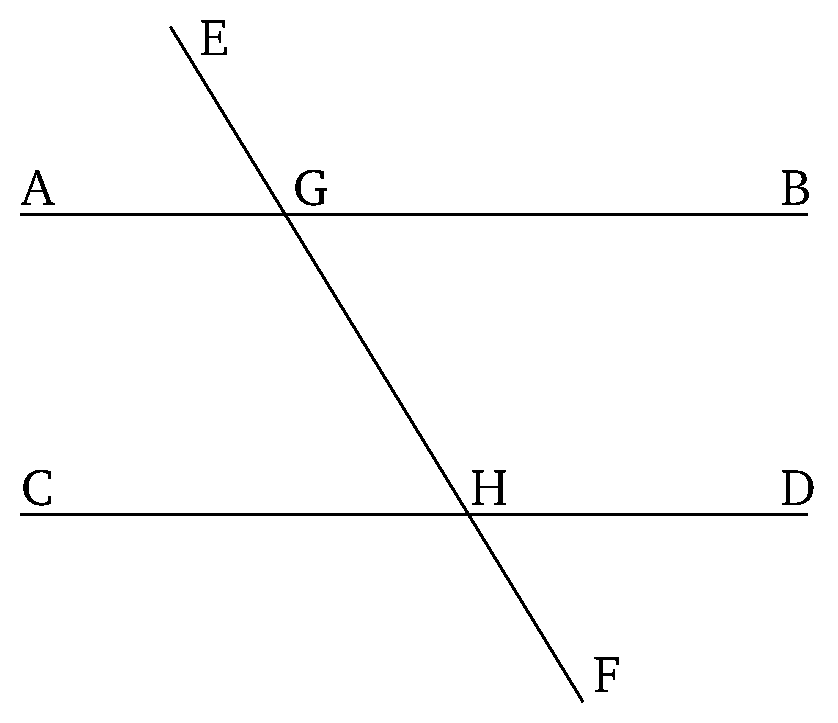
\includegraphics[width=0.5\linewidth]{figures/fig28e.eps}
    \label{fig:prop_28}
    \end{center}
\end{figure*}

If a straight-line falling across two straight-lines makes the external angle equal
to the internal and opposite angle on the same side, or (makes) the (sum  of the) internal
(angles) on the same side equal
to two right-angles, then the (two) straight-lines will be parallel to
one another.

For let $EF$, falling across the two straight-lines $AB$ and $CD$, make the external
angle $EGB$ equal to the internal and opposite angle $GHD$, or the (sum of the) internal
(angles) on the same side, $BGH$ and $GHD$, equal to two right-angles.
I say that $AB$ is parallel to $CD$.

For since (in the first case) $EGB$ is equal to $GHD$, but $EGB$ is equal to $AGH$ [Prop.~1.15],
$AGH$ is thus also equal to $GHD$. And they are alternate (angles).
Thus, $AB$ is
 parallel to $CD$ [Prop.~1.27].
 
Again, since (in the second case, the sum of) $BGH$ and $GHD$ is equal to two right-angles,  and (the sum of) $AGH$ and
$BGH$ is also equal to two right-angles [Prop.~1.13], 
(the sum of) $AGH$ and $BGH$ is thus equal to (the sum of) $BGH$ and $GHD$. Let $BGH$ have been
subtracted from both. Thus, the remainder $AGH$ is equal to the remainder
$GHD$. And they are alternate (angles). Thus, $AB$ is parallel
to $CD$ [Prop.~1.27].

Thus, if a straight-line falling across  two straight-lines makes the external angle equal
to the internal and opposite angle on the same side, or (makes) the (sum of the) internal
(angles) on the same side equal
to two right-angles, then the (two) straight-lines will be parallel (to
one another). (Which is) the very thing it was required to show.


\section*{Commentary}

\begin{proposition}\label{proposition_28}\lean{Elements.Book1.proposition_28}\leanok
    $A$ and $B$ are two distcint points on $AB$. $C$ and $D$ are two distinct points on $CD$. $E$ and $F$ are two distinct points on $EF$. $G$ is between $A$ and $B$. $H$ is between $C$ and $D$. $G$ is between $E$ and $H$. $H$ is between $G$ and $F$. $B$ and $D$ are on the same side of $EF$. Either $\angle~EGB = \angle~GHD$ or $\angle~BGH + \angle~GHD = \pi$. Then, $AB$ and $CD$ must be parallel.
\end{proposition}
\begin{proof}
    \uses{proposition_13,proposition_15,proposition_27}\leanok
    See the original proof by Euclid.
\end{proof}
